\clearpage
\section*{Question 4}
\addcontentsline{toc}{section}{Question 4}

	\textbf{Question:} \\ 
Find the system eigenvalues using the MATLAB functions \texttt{linmod} and \texttt{eig} on the command line. Compare the results with part 2.

\subsection*{MATLAB Output}
The following figure shows the eigenvalues computed using MATLAB's \texttt{linmod} and \texttt{eig} functions:
\begin{figure}[H]
	\centering
	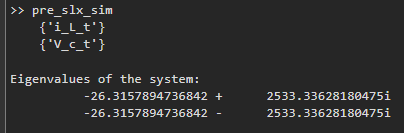
\includegraphics[width=0.6\textwidth]{figures/hw01_q04_eigen-values-via-matlab-linmod-and-eig.png}
	\caption{Eigenvalues of the system computed using \texttt{linmod} and \texttt{eig} in MATLAB.}
\end{figure}

\subsection*{Comparison with Analytical Results}
The eigenvalues obtained from MATLAB are:
\begin{align*}
	&-26.3158 \pm 2533.34i
\end{align*}
These match very closely with the hand-computed values in Q2:
\begin{align*}
	&-26.316 \pm 2533.3i
\end{align*}
The small numerical difference is due to rounding and floating-point precision in MATLAB. Both methods confirm the system is underdamped with complex conjugate eigenvalues, as expected from the analytical derivation.


